% !TEX TS-program = pdflatex
% !TEX encoding = UTF-8 Unicode

\documentclass{article}

\usepackage{kotex}
\usepackage{graphicx}
\usepackage{subfigure}
\usepackage{amsmath}
\usepackage{pict2e}
\usepackage[onehalfspacing]{setspace}
\usepackage[a4paper,left=35mm,right=35mm,top=40mm,bottom=40mm]{geometry}

\newcommand{\wdcbsd}{
  \begingroup
  \setlength{\unitlength}{\fontcharht\font`T}
  \begin{picture}(1,1)
  \polygon(.5,0)(1,.5)(.5,1)(0,.5)
  \polygon*(.5,0.2)(.8,.5)(.5,.8)(.2,.5)
  \end{picture}
  \endgroup
}

\newcommand{\Lim}[1]{
	\raisebox{0.5ex}{\scalebox{0.8}{$\displaystyle \lim_{#1}\;$}}
}

\begin{document}

\title{프로그래밍 언어 HW0}
\author{B743014 양혜진}
\date{\today}
\maketitle

\section{자기소개}
안녕하세요 저는 홍익대학교 미술대학 금속조형디자인과 3학년에 재학중인 양혜진입니다.
저는 안드로이드 앱을 만들기 위해 프로그래밍을 공부하다가 컴퓨터 공학 분야에 관심을
갖게 되어 컴퓨터공학과를 복수전공하고 있습니다. 지금까지는 Kotlin을 사용해서 Android
앱 개발을 주로 해 왔으나, 올해 애플의 교육프로모션으로 맥북을 구입하게 되면서 iOS
개발에 관심을 가지게 되었습니다. 그래서 현재 컴퓨터공학과 개발 학회 SODA 에
들어가서 만난 사람들과 iOS 개발 스터디를 진행하고 있습니다. 이번 여름방학에는
저만의 iOS 앱을 만들어서 앱스토어에 출시해보고 싶습니다.

\section{수식작성: 미분계수}
\begin{list}{$\wdcbsd$}{}
	\item 함수 $f(x)$의 $x=a$에서의 미분계수
	\begin{list}{--}{}
		\item 함수 $y=f(x)$에서 $x$의 값이 $a$에서 $a+h$까지 변할 때,
			$x$의 증분 $\Delta x\to 0$일 때 평균변화율의 극한값이 존재하면
			이 극한값을 함수 $y=f(x)$의 $x=a$에서의 순간변화율 또는 미분계수라고 한다.
		\item $ \begin{aligned}[t] & f^\prime(a)=\Lim{\Delta x\to0}\frac{\Delta y}{\Delta x}\\[8pt]
			  & = \Lim{h\to0}\frac{f(a+h)-f(a)}{h}\\[8pt]
			  & = \Lim{x\to a}\frac{f(x)-f(a)}{x-a} \end{aligned}$
	  \end{list}
	\item 미분계수의 기하학적 의미
	\begin{list}{--}{}
		\item 함수 $f(x)$의 $x=a$에서의 미분계수 $f^\prime(a)$는
			곡선 $y=f(x)$ 위의 점 $(a,f(a))$에서의 접선의 기울기를 나타낸다.
	\end{list}
	\item 미분가능성과 연속성
	\begin{list}{--}{}
		\item 함수 $f(x)$가 $x=a$에서 미분가능하면 $y=f(x)$는 $x=a$에서 연속이다.
	\end{list}
\end{list}

\newpage

\section{가장 좋아하는 그림}
\label{sec:sec3}
\begin{figure}[!htbp]
	\begin{center}
		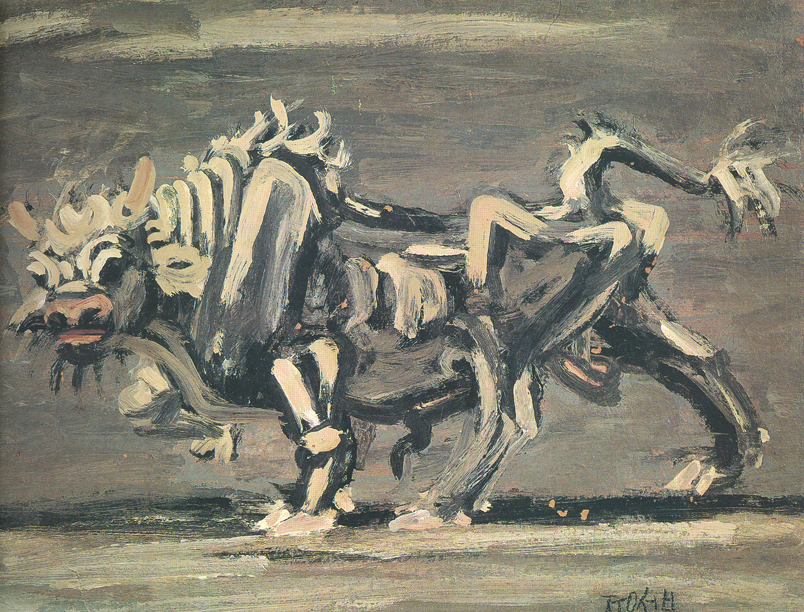
\includegraphics[width=230pt]{WhiteOx}
		\caption{이중섭, $<$흰 소$>$, 1954. 종이에 유채, 30x41.7cm. 한국, 홍익대학교박물관}
	\end{center}
	\label{fig:fig1}
\end{figure}

\subsection{나를 나타낼 수 있는 사진}
\label{sec3:subsec1}
\begin{figure}[!htbp]
	\begin{center}
		
\includegraphics[width=250pt]{Block}
		\caption{장난감 블록 이미지}
	\end{center}
	\label{fig:fig2}
\end{figure}
\noindent 저는 장난감 블록(Figure~\ref{fig:fig2}) 같은 사람입니다. 저는 정해진 규칙 아래에서 행동하는 것을 좋아합니다.
그래서 저의 모습이 마치 우직한 소와 같다는 이야기를 듣기도 합니다. 그래서 홍익대학교 박물관에 소장되어 있는 이중섭의
$<$흰 소$>$그림(Figure~\ref{fig:fig1})은 제가 가장 좋아하는 그림 중 하나입니다. 또한, 장난감 블록을 여러개 쌓으면 무엇이든지
만들 수 있듯이 저는 규칙적이고 단조로운 삶 속에서도 무언가 새로운 것을 발견하고 창조적인 활동을 하는 것을 즐깁니다.

\subsection{좋아하는 연예인 사진}
\label{sec3:subsec2}
\begin{figure}[!htbp]
	\begin{center}
		\subfigure[정우성 1]{
\includegraphics [width = 0.51\textwidth]{JWS}}
		\subfigure[정우성 2]{
\includegraphics [width = 0.29\textwidth]{JWS2}}
		\caption{영화배우 정우성}
	\end{center}
	\label{fig:fig3}
\end{figure}
\noindent 사실 저는 연예인에 큰 관심이 없기 때문에 좋아하는 연예인이 없습니다. 하지만 그럼에도 연예인 중에서 제일 좋아하는 한 명을 골라야 한다면,
저는 영화배우 정우성을 고를 것입니다. 왜냐하면 영화배우 정우성씨가 매우 잘생겼다고 생각하기 때문입니다. 저는 영화배우 정우성씨를 영화 $<$감시자들$>$에서
처음 알게되었습니다. 그 때 정우성씨가 참 잘생겼다고 생각했었는데, 우연히 정우성씨가 주연으로 나온 1997년 영화 $<$비트$>$(Figure~\ref{fig:fig3} (a))를 보고
'젊으셨을떄는 더 잘생기셨구나'라고 생각하게 되었습니다. 하지만 영화 $<$비트$>$를 촬영한지 약 24년이 지난 지금에도 영화배우 정우성씨는
중후한 중년미(Figure~\ref{fig:fig3} (b))를 풍기게 되며 더 잘생겨지신 것 같습니다.

\end{document}

%------------------------------------------------